% !TEX root = ../thesis.tex

\begin{figure}
  \def\fibfigsize{1\linewidth}
  \centering
  \begin{subfigure}{\fibfigsize}
    \caption{Starting of the streaming process using a WPS \emph{Execute} request, requesting of the streaming process's description and supplying of three input messages, of which only $fib(0) = 0$ can be processed immediately.}
    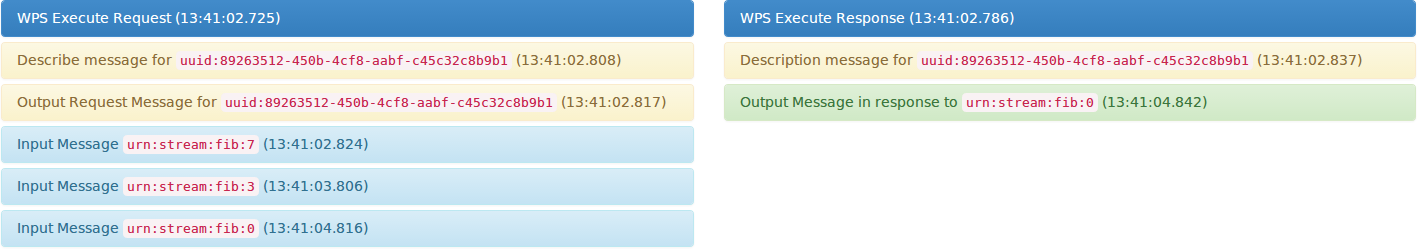
\includegraphics[width = \linewidth]{figures/fibonacci-1.png}
  \end{subfigure}
  \begin{subfigure}{\fibfigsize}
    \caption{$fib(1) = 1$ is supplied in an input message, and so the previously supplied request for $fib(2)$ and $fib(3)$ can be calculated. $fib(7)$ is still missing prerequisites.}
    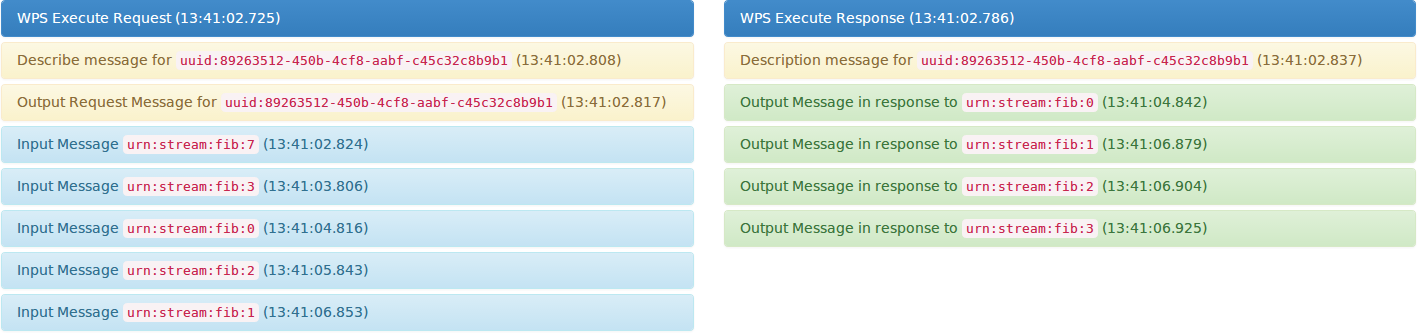
\includegraphics[width = \linewidth]{figures/fibonacci-2.png}
  \end{subfigure}
  \begin{subfigure}{\fibfigsize}
    \caption{As the dependencies of $fib(4)$ and $fib(5)$ are fulfilled, they can directly be calculated. $fib(7)$ is still missing the result of $fib(6)$.}
    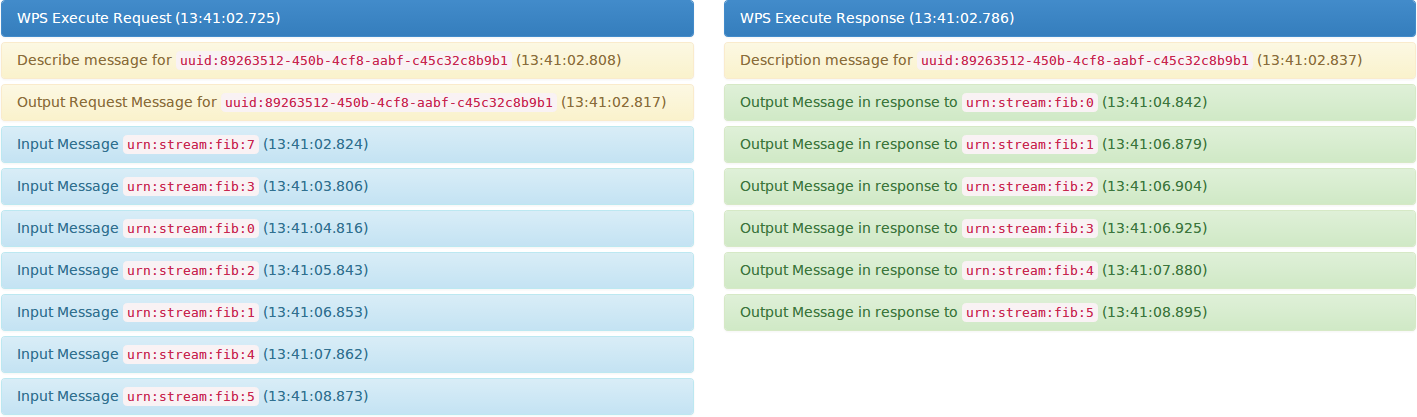
\includegraphics[width = \linewidth]{figures/fibonacci-3.png}
  \end{subfigure}
  \begin{subfigure}{\fibfigsize}
    \caption{At the time the request for $fib(6)$ arrives, all preconditions are met and $fib(6)$ and the final $fib(7)$ can be calculated. Once the result has arrived, the client stops the streaming process.}
    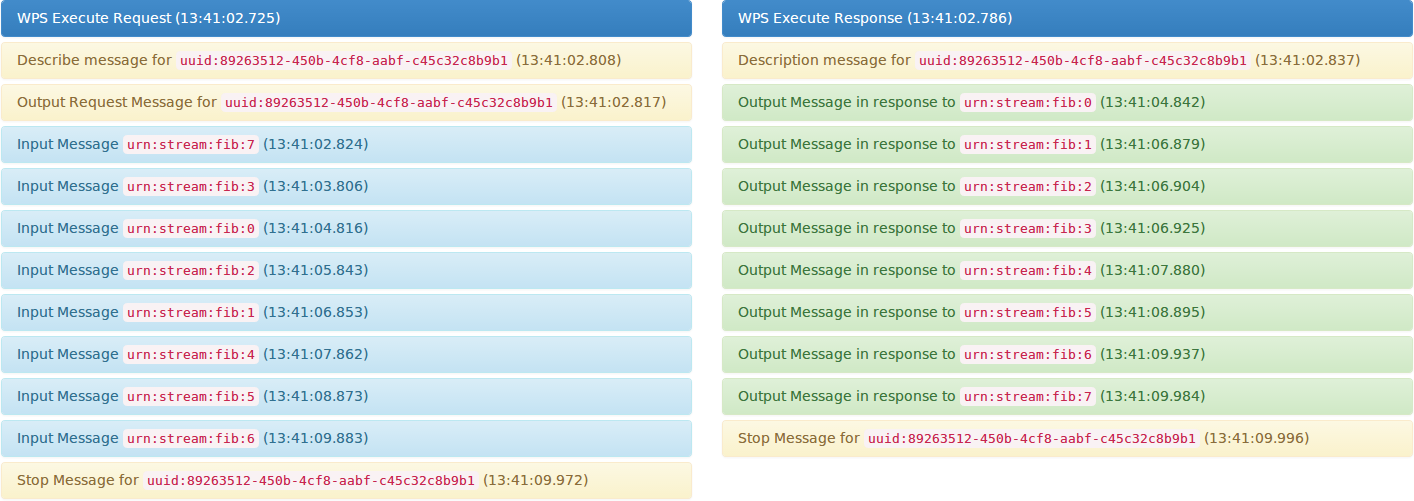
\includegraphics[width = \linewidth]{figures/fibonacci-4.png}
  \end{subfigure}
  \caption{\label{fig:client}Calculation of the seventh Fibonacci number using the Streaming WPS, its accompanying JavaScript API and a simple addition WPS process as the streaming process's delegate.}
\end{figure}